\documentclass{article}

\title{Project Proposal EL2320}
\author{Axel Lundin (axlundin) and Andrea Gnoato (gnoato)}
\usepackage{graphicx}

\setlength{\parindent}{0pt}

\begin{document}

\maketitle

\section*{Consice description}

We propose to implement EKF-SLAM on the bonirob dataset. This dataset contains several rosbags of sensor readings from three LiDARs and two GPS mounted to a agricultural robot used to monitor crop growth of sugar beets. \\ 

The scope of the project is to (i) process the data, (ii) implement the SLAM algorithm and (iii) visualize the result. The goal of the project is to build a map of the environment and estimate a trajectory of the robot. There are additional sensors on the robot that are used for crop monitoring, which will not be of interest in this project. The robot used for data collection is shown in Figure \ref{fig:bonirob_robot}.

\begin{figure}
    \centering
    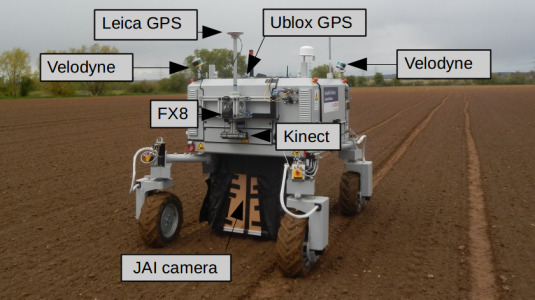
\includegraphics[width=0.6\textwidth]{bonirob.jpg}
    \caption{The robot used in the dataset.}
    \label{fig:bonirob_robot}
\end{figure}

\section*{Difficulties}

We believe that the difficulties in the project will arise from choosing a subset of the data to work with (there is 5TB of data), and effectively combining measurements from all the sensors. Another problem might be the self similarity of the field environment, which might pose a difficulty for the localization problem. 


\end{document}
